\section{Base Technologies of Clouds}
\subsection{Process Technology}
\paragraph{Production} the processors are produced from semi-conductor materials. It's primarily produced on a \textbf{waver} consisting of a lot of chips. Later the waver is cut after the production process. Individual chips will be packaged into the system.

\paragraph{Transistor} 
\begin{itemize}
	\item traditional 2D planar transistor: a 2D-planar structure, the gate controls how much current flows from source through the drain.
	\item 3D tri-gate transistor \textbf{FinFET}: conducting channels on 3 sides with a \textbf{vertical fin structure}. The width of a Fin is \textbf{10nm}, and it keeps shrinking.
\end{itemize}
The smaller the structure gets, the more transistors fit on the same space, the faster the transistor gets.

\subsection{Processor Architecture}

\subsubsection{CPU}
\begin{itemize}
	\item current state of CPU development:
	\begin{itemize}
		\item increase in transistors: up to 10nm or even 5nm.
		\item stop in increase of clock speed: up to 4GHz. Limitation: cooling. (the faster the clock speed, the more energy consumed, the hotter) 
		\item continuous need of performance improvement: parallelism on the chip, since halt in clock speed.
	\end{itemize}
	\item trends in CPU development:
	\begin{itemize}
		\item multi-core processors: parallelism
		\item SIMD support (Single Instruction, Multiple Data): parallelism inside of a single instruction, computation of vectors of values in parallel.
		\item combination of core private and shared caches:
		\begin{itemize}
			\item data saved in cache for repeated operations
			\item with multiple caches, cores can communicate. However, this may disturb the usage of cache.
			
		\end{itemize}
		\item hardware support for energy control: \textbf{dynamic voltage and frequency scaling}  
		\begin{itemize}
			\item chips work in a dynamic frequency controlled by hardware according to the need of the running software. 
			\item It checks whether operations are memory-bound or compute-bound.
		\end{itemize}
		   
		\item 64-bit architectures
		  
	\end{itemize}
	\item challenge: the \textbf{memory hierarchy}
	\begin{itemize}
		\item access to the main memory is slow, involving several hundreds of cycles for CPU, while each of these cycles can be responsible for multiple operations.
		
		$\rightarrow$ save such cycles for accessing data but keep the \textbf{data near to execution}.
		\item \textbf{Level-1 Instruction \& Data Cache}: fastest, but too slow to feed all data in large size. (64 Bytes: 8 double precision values, 64 bit long values)
		\item \textbf{Level-2 Unified Cache}: not separated, access better. 
		\item \textbf{Translation Lookaside Buffer (TLB)}: translates virtual addresses into physical addresses and loads into main memory, it only stores the \textbf{most recent translation}, no need to lookup constantly.
	\end{itemize}
	\begin{figure}[H]
		\centering
		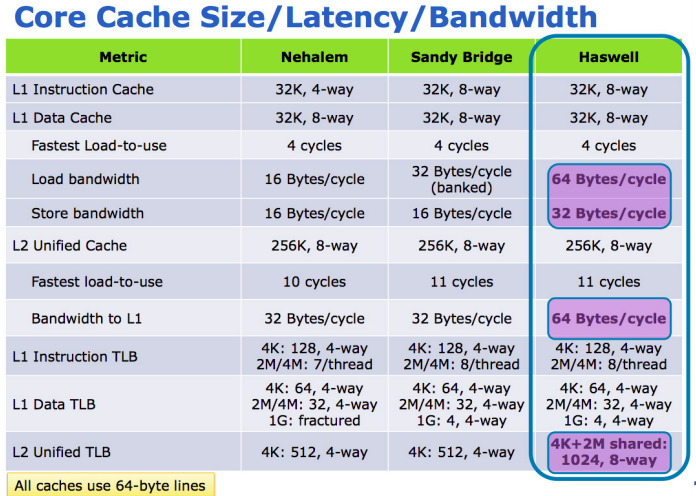
\includegraphics[width=0.65\textwidth]{memhier.png}
	\end{figure}
\end{itemize}

\subsubsection{Skylake Architecture} 

\begin{figure}[H]
	\centering
	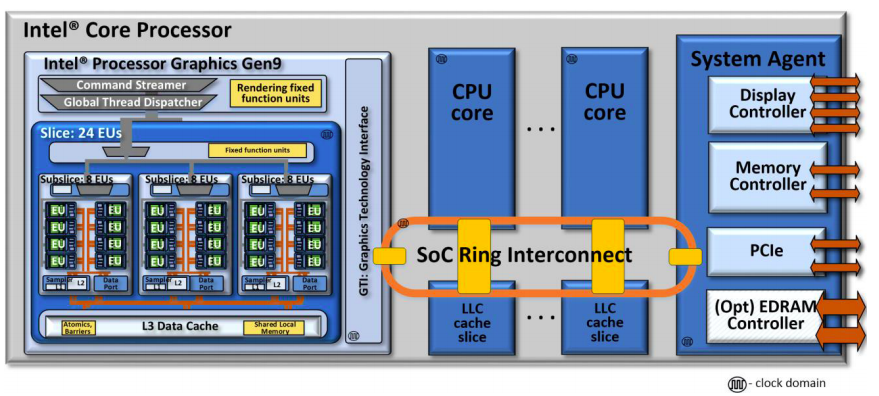
\includegraphics[width=0.7\textwidth]{skylake.png}
\end{figure}
The archiecture of a processor (one chip)
\begin{itemize}
	\item graphic processor: accelerator for specified computation
	\item system agent: support structures (eg: display controller, memory controller, PCIe for I/O, EDRAM controller)
	\item CPU cores: homogeneous cores with a \textbf{private cache each}.
	\item LLC cache slice: each slice cache is associated to each CPU core. 
	\begin{itemize}
		\item If core misses information in its private cache: through interconnect, it checks which slice cache contains the info, then it propagates to the cache associated the CPU core and returns the info back to the CPU.
	\end{itemize}
	
	\item SoC Ring interconnect: all parts are connected by a ring bust.
	\begin{itemize}
		\item if CPU writes to I/O device -- PCIe, it first puts information onto the bust, then it propagates into the PCIe and is written to the disk.
	\end{itemize}
\end{itemize}
$\rightarrow$ the \textbf{interconnect ring} is the \textbf{bottleneck} for increasing the cores.

$\rightarrow$ alternatives: Xeon Phi

\subsubsection{Xeon Phi Architecture} 
\begin{figure}[H]
	\centering
	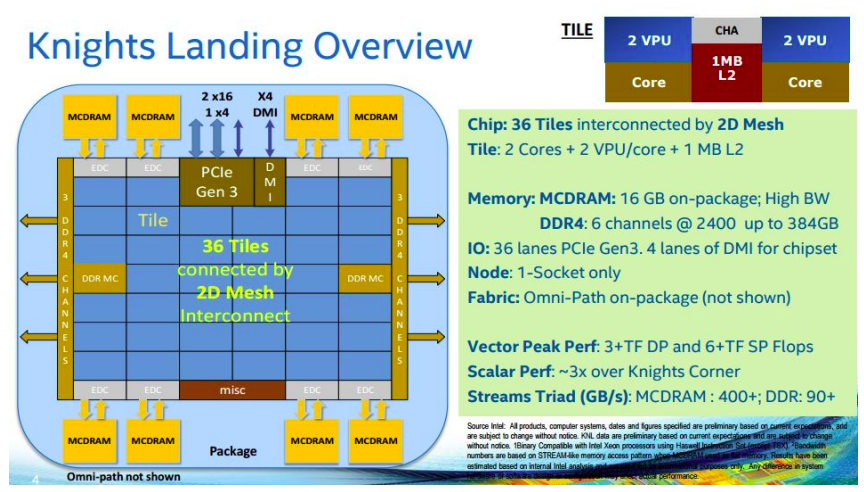
\includegraphics[width=0.7\textwidth]{xeonphi.png}
\end{figure}
\begin{itemize}
	\item Goal: allows significantly \textbf{more cores} in a single processor, in a single CPU die.
	\item Idea: 
	\begin{itemize}
		\item the die is organized into a \textbf{tile-architecture}.
		\item 36 compute tiles are connected through a \textbf{2D mesh network} $\rightarrow$ connection between tiles in both x- and y-direction.
		\item each tile has 2 cores $\rightarrow$ \textbf{72 cores} in total
	\end{itemize}
	\item Tile structure:
	\begin{itemize}
		\item 2 cores
		\item 2 VPUs (Vector Processing Unit) for each core $\rightarrow$ 4 in total per tile.
		\item L2 cache: shared between the cores, but as a private cache for each tile. 
		
		$\rightarrow$ multiple copies of an address can be in different private L2 caches of different tiles, which \textbf{must be coherent}.
		\item CHA (Caching Hold Agent): responsible for the \textbf{coherence}. It's connected to each tile, keeping track of the status of the copies by implementing a \textbf{coherence protocol}. 
	\end{itemize}
	\item Memory: 
	\begin{itemize}
		\item DDR4 memory
		\item \textbf{MCDRAM}-- Multi-channel DRAM, \textbf{high bandwidth}(450 GB/s)
		
		Memory modes:
		\begin{itemize}
			\item flat mode: all MCDRAM is used as \textbf{physical address}. Data structure can explicitly choose between MCDRAM or DDR. 
			\item cache mode: all MCDARM is used as \textbf{L3 cache}. physical addresses only on DDR. If data is being processed from DDR, it's mapped to MCDRAM.
			\item hybrid mode: combination of flat and cache mode. Part of MCDRAM is used as \textbf{L3 cache}, the other as \textbf{physical addresses}.
		\end{itemize}
		\begin{figure}[H]
			\centering
			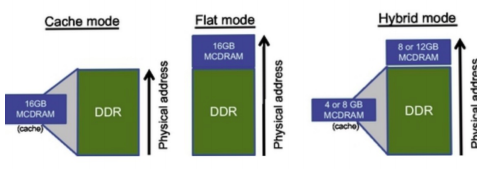
\includegraphics[width=0.65\textwidth]{memorymodes.png}
		\end{figure}
	\end{itemize}	
\end{itemize}

\subsubsection{Processors for mobile devices: ARM}
\begin{figure}[H]
	\centering
	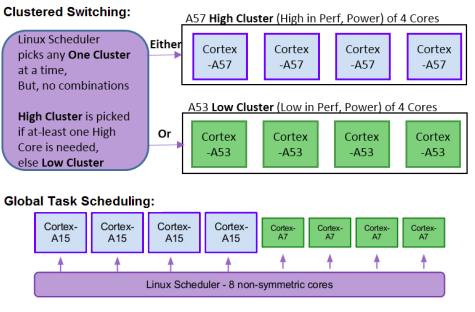
\includegraphics[width=0.65\textwidth]{arm.png}
\end{figure}
\begin{itemize}
	\item \textbf{Big Little Principle}
	\begin{itemize}
		\item Combination of \textbf{high clusters} and \textbf{low clusters}, controlled by clustered switching. 
		\begin{itemize}
			\item high cluster: high in performance
			\item low cluster: low in performance, but energy efficient
			\item only \textbf{one cluster} at a time, \textbf{no combinations}.
		\end{itemize}
		\item Global task scheduling: tasks are scheduled according to the requirement between 2 clusters.
	\end{itemize}
	\item Use-cases: Apple Processor A14 (2 high performance Firestorm, 2 energy-efficient Icestorm)
\end{itemize}


\subsection{Accelerator Programming}
\begin{itemize}
	\item Motivation: 
	\begin{itemize}
		\item increase computational speed and reduce energy consumption
		
		$\rightarrow$ achieved by \textbf{specialization} in operations/on-chip communication/memory accesses
		
		$\rightarrow$ \textbf{accelerator}
	\end{itemize}
	\item Types:
	\begin{itemize}
		\item GPGPU (General Purpose Graphic Processors)
		\item FPGA
		\item standard cores
	\end{itemize}
	\item Designs:
	\begin{itemize}
		\item CPU with accelerators attached: computation can be offloaded onto the accelerator.
		\item accelerators-only design
		\item accelerator booster: a collection of accelerators as a separate part from the whole system. Jobs can be computed by these accelerators when necessary. Accelerator booster can be shared among parallel jobs.
	\end{itemize}
	
\end{itemize}

\subsubsection{Graphic Processing Units (GPU)}
\begin{itemize}
	\item Usage: 
	\begin{itemize}
		\item visualization
		\item \textbf{general processing} (NVIDIA)
	\end{itemize}
	\item Parallelism: multi-threading, MIMD, SIMD
	\item Challenges:
	\begin{itemize}
		\item a \textbf{specialized programming interface} for the GPGPU needed (eg: CUDA from NVIDIA)
		\item \textbf{scheduling coordination} on system processor and GPU
		\item \textbf{transfer of data} between system memory and GPU memory
	\end{itemize} 
	\item example: NVIDIA Tesla P100
\end{itemize}

\paragraph{NVIDIA Tesla P100}
\begin{itemize}
	\item GP100 (GPU):
	\begin{itemize}
		\item L2 cache: shared among all compute units --  streaming multi-processor
		\item NVLink: able to connect multiple GPGPUs together
		\item memory controller: access to high bandwidth memory
		\item 6 Graphic Processing Clusters(GPC)
			\begin{itemize}
				\item 10 Streaming Multi-Processor each GPC, 60 in total
				\item 5 Textural Processing Clusters (TPC), 1 for 2 SM, 30 in total
			\end{itemize}
		\end{itemize}

		\item High Bandwidth Memory (HBM)
		\begin{itemize}
			\item \textbf{vertical stacks} of memory dies connected by microscopic wires
		
			$\rightarrow$ near and tight connection between memories
			\item 180 GB/s per stack bandwidth
		\end{itemize}
\end{itemize}

$\rightarrow$ good for data parallel processing like vector processing.

\subsubsection{Field Programmable Gate Arrays (FPGA)}
\begin{itemize}
	\item hardware which is programmable
	\item Consist of:
	\begin{itemize}
		\item \textbf{array of logic gates} to implement \textbf{hardware-programmed special functions}
		\item \textbf{specialized functional units} (eg: signal processors, multipliers)
		\item static \textbf{memory}
	\end{itemize}
	\item programmed in VHDL: the program describe functions to be executed, it will then be translated into look-up tables, which are put into the logic gates
	\item Use-case:
	\begin{itemize}
		\item as \textbf{accelerator} for specialized computations
		\item \textbf{filtering} for databases
		\item as \textbf{switches, routers} for communication
		\item \textbf{preprocessing}: I/O hardware of FPGA accesses the DDR, local computation can be organized in the pipeline of FPGA. Local preprocessing will be done on FPGA and the output will be sent ot external processor via PCIe.
	\end{itemize}
	\item examples: Altera, Xilinx
\end{itemize}

\subsection{Architecture for Parallelism: Shared Memory Systems}
\begin{itemize}
	\item Idea: 2 architectures to \textbf{achieve parallelism}, which is combining multiple processors together for computation. 
	\begin{itemize}
		\item shared memory system
		\item distributed memory system
	\end{itemize}
	\item \textbf{Non-Uniform Memory Access (NUMA)}:
	\begin{itemize}
		\item \textbf{multiple CPU} with multiple cores are connected through \textbf{single physical address} space.
		
		$\rightarrow$ access time depends on the \textbf{distance to the physical address} (memory)
		
		$\rightarrow$ CPU accesses either local(near) or remote memory $\rightarrow$ locate the memory near for fast access.
	\end{itemize}
	\paragraph{Example: SuperMUC}
	
	\begin{itemize}
		\item 2 multi-core processors(Sandy Bridge) with 32GB memory in total
		\item each processor can access to all 32GB memory, \textbf{however access time differs}
		\item \textbf{Latency}
		\begin{itemize}
			\item local: $\sim$50ns, $\sim$135 cycles
			\item remote: $\sim$90ns, $\sim$240 cycles
		\end{itemize}
		
	\end{itemize}
	\begin{figure}[H]
		\centering
		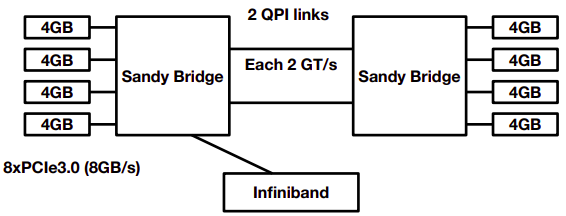
\includegraphics[width=0.65\textwidth]{numa.png}
	\end{figure}

	\item Programming interfaces for Shared Memory Systems
	\begin{itemize}
		\item explicit threading
		\item automatic parallelization: sequential code is given to compiler, which \textbf{automatically} parallelize the work among available CPUs.
		\item OpenMP: directive-based parallel programming, parallel computations are \textbf{explicitly expressed}.
	\end{itemize}
	\item Challenges in parallel computing:
	\begin{itemize}
		\item explicit synchronization needed.
		\item \textbf{cocurrency bugs}: the outcome of the computation depends on the speed of access to the memory $\rightarrow$ non-deterministic results possible.
		\item control of \textbf{data locality}
	\end{itemize}
\end{itemize}

\subsection{Architecture for Parallelism: Distributed Memory Systems}
\begin{itemize}
	\item Characteristics
	\begin{itemize}
		\item \textbf{Coupling} of individual nodes via network: processor only have access to the memory in node.
		\item \textbf{no shared} physical address space
		\item communication between nodes: transfer of \textbf{messages}
	\end{itemize}
	\item Programming in Distributed Memory Systems: \textbf{more difficult} than shared memory systems.
	\begin{itemize}
		\item + : \textbf{rare race conditions} $\rightarrow$ cocurrency bugs low.
		\item -- : Message Passing Interface(MPI), have to explicitly decompose or insert message passing $\rightarrow$ more difficult to program.
		\item Process to Process communication and collective operations
	\end{itemize}
	\item Challenges: 
	\begin{itemize}
		\item \textbf{more difficult} to programm than shared memory systems
		\item \textbf{expensive communication}, much slower than access to memory.
		$$t(message) = \text{startup time} + \frac{\text{message size}}{\text{bandwidth}}$$
		\begin{itemize}
			\item communication with one large message is more efficient than multiple small messages (startup time)
			\item mapping onto processors has performance impact. Communication may not need to go through the entire but locally. (eg: 2D mesh network)
		\end{itemize}
	\end{itemize}
\end{itemize}

